%   Copyright (c) 2002 Software in the Public Interest, Inc.
%
%   This program is free software; you can redistribute it and/or modify
%   it under the terms of the GNU General Public License as published by
%   the Free Software Foundation; version 2 dated June, 1991.
%
%   This program is distributed in the hope that it will be useful,
%   but WITHOUT ANY WARRANTY; without even the implied warranty of
%   MERCHANTABILITY or FITNESS FOR A PARTICULAR PURPOSE.  See the
%   GNU General Public License for more details.
%
%   You should have received a copy of the GNU General Public License
%   along with this program;  if not, write to the Free Software
%   Foundation, Inc., 59 Temple Place - Suite 330, Boston, MA 02111, USA.

%% Layout for a Debian Flyer
%% By Jens Schmalzing <jensen@debian.org> and 
%% Michael Banck <mbanck@debian.org>

% some definitions, for brevity
\setlength{\Separation}{.02\textwidth}
\def\Itemizesymbol{\item[\textcolor{debianred}{$\blacktriangleright$}]}
\def\Descriptionsymbol{\item[\hspace{-\Separation}\textcolor{debianred}{$\blacksquare$}\hspace{.5\Separation}}
\definecolor{debianred}{rgb}{0.843137,0.027451,0.317647}

\def\Sponsor{%
\vspace*{\stretch{1}}
\vspace*{-14mm}
\hbox to\textwidth{%
  \hbox to0.44\textwidth{%
    \null\hspace{\Separation} \MadeWith \hfill}
  \hfil%
  \parbox{0.40\textwidth}{\raggedleft%
      \SponsoredBy \\
      \expandafter\boxurl\SponsorURL
  }
  \hspace*{0.5\Separation}\null
  \lower8.5pt\hbox{\includegraphics[width=0.1\textwidth]{\SponsorLogo}}
}
\vspace*{1mm}
}

\raggedleft

% a tiny minipage for the background swirl
\begin{minipage}{.01\textwidth}
%\MyRCS

\includegraphics[width=100.\textwidth]{swirl}
\end{minipage}
%
\hfill
%
% another minipage for everything else
\begin{minipage}{.98\textwidth}
%
% some rules around the text
\hspace{-\Separation}%
\smash{\rule[-\textheight]{1pt}{\textheight}}%
\hspace{-1pt}%
\rule{1.04\textwidth}{1pt}%
% Beware, below is a hack (tm). It might be better to use a
% \begin{picture}(0,0) construct to draw the lines around the text
\hbox to0pt{\raise1pt\vbox to0pt{\rule{1pt}{\textheight}%
\hskip-1.04\textwidth\rule[-1pt]{1.04\textwidth}{1pt}\rule[-1pt]{0.4pt}{1pt}%
\vss}\hss}%

\vspace*{\Separation}
%
\begin{minipage}{.39\textwidth}
\resizebox*{\textwidth}{!}{\colorbox{debianred}{\color{white}\bf \WhatIsDebianCaption}}

\vspace*{\Separation}

\WhatIsDebian
\end{minipage}
%
\hfill
%
\begin{minipage}{.59\textwidth}
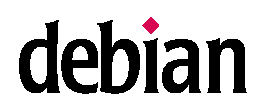
\includegraphics[width=\textwidth]{debian} \\[1ex]
\resizebox*{\textwidth}{!}{\bf \Universal}
\end{minipage}

\vspace*{\Separation}

\hspace{-\Separation}%
\rule{1.04\textwidth}{1pt}

\vspace*{\Separation}

\begin{minipage}[t]{.44\textwidth}
%
\begin{description}\itemsep0cm
\Descriptionsymbol\FreedomCaption] \Freedom
\Descriptionsymbol\ContinuityCaption] \Continuity
\Descriptionsymbol\SecurityCaption] \Security
\Descriptionsymbol\QualityCaption] \Quality
\end{description}
%
\end{minipage}
%
\hfill
%
\begin{minipage}[t]{.54\textwidth}
%
\colorbox{debianred}{\textcolor{white}{\bf\Large \IncludedCaption}}

\vspace*{\Separation}

\Included
\begin{itemize}\itemsep0cm
\Itemizesymbol\Utilities
\Itemizesymbol\Networking
\Itemizesymbol\Programming
\Itemizesymbol\Windowsystem
\Itemizesymbol\Documents
\Itemizesymbol\Graphics
\Itemizesymbol\Office
\Itemizesymbol\Databases
\end{itemize}
%
\colorbox{debianred}{\textcolor{white}{\bf\Large \KnowMoreCaption}}

\vspace*{\Separation}

\KnowMore

\Install

\end{minipage}

\end{minipage}

\Sponsor

